\documentclass{fank1basedocument}

\usepackage{fank1code}
\usepackage{graphicx}
\usepackage{hyperref}
\usepackage{titlesec}

\settitle{Code Smell Refactorings (Summit)}

\fancyhead[L]{CSSE375}
\fancyhead[R]{Spring 2024-2025}

\begin{document}

\tableofcontents

\addcontentsline{toc}{section}{Duplicate Code (Milestone 2)}
\section*{Duplicate Code (Milestone 2)}
\subsection*{Description}
In \texttt{Adjacency}, there is duplicated code when initializing the maps containing information on which tiles, roads, settlements, and ports are adjacent. For each type of adjacency, there is a method for adding the adjacent location information to the adjacency map, and the process for adding the information is similar. The code could be improved by reading the adjacency information from a file and using loops to add the information to the maps because the adjacency information does not change between games. Also, since the process for adding the information is similar, we can use polymorphism to create an initializer for setting up each type of adjacency map.
\subsection*{Before}
\begin{lstlisting}[style=javacode,language=myJava]
public class Adjacency {
	private Map<Location, Set<Location>> roadToRoads;
	private Map<Location, Set<Location>> roadToSettlements;
	private Map<Location, Set<Location>> settlementToSettlements;
	private Map<Location, Set<Location>> tileToTiles;
	private Map<Location, Location> settlementToPort;

	public Adjacency() {
		this.initializeRoadToRoads();
		this.initializeRoadToSettlements();
		this.initializeSettlementToSettlements();
		this.initializeTileToTiles();
		this.initializeSettlementToPorts();
	}
		
	private void initializeRoadToSettlements() {
		this.roadToSettlements = new HashMap<>();

		// ROW ONE
		this.mapRoadToSettlements('r', 'A', 'q', 'a');
		this.mapRoadToSettlements('a', 'A', 'r', 'B');
		this.mapRoadToSettlements('a', 'B', 'A', 'b');
		this.mapRoadToSettlements('b', 'B', 'a', 'C');
		this.mapRoadToSettlements('b', 'C', 'B', 'c');
		this.mapRoadToSettlements('c', 'C', 'b', 'd');

		// ROW TWO
		this.mapRoadToSettlements('q', 'A', 'D', 'r');
		this.mapRoadToSettlements('A', 'B', 'E', 'a');
		this.mapRoadToSettlements('B', 'C', 'F', 'b');
		this.mapRoadToSettlements('C', 'd', 'G', 'c');

		// ROW THREE
		this.mapRoadToSettlements('q', 'D', 'p', 'A');
		this.mapRoadToSettlements('A', 'D', 'q', 'E');
		this.mapRoadToSettlements('A', 'E', 'D', 'B');
		this.mapRoadToSettlements('B', 'E', 'A', 'F');
		this.mapRoadToSettlements('B', 'F', 'E', 'C');
		this.mapRoadToSettlements('C', 'F', 'B', 'G');
		this.mapRoadToSettlements('C', 'G', 'F', 'd');
		this.mapRoadToSettlements('d', 'G', 'C', 'e');

		// ROW FOUR
		this.mapRoadToSettlements('p', 'D', 'H', 'q');
		this.mapRoadToSettlements('D', 'E', 'I', 'A');
		this.mapRoadToSettlements('E', 'F', 'J', 'B');
		this.mapRoadToSettlements('F', 'G', 'K', 'C');
		this.mapRoadToSettlements('G', 'e', 'L', 'd');

		// ROW FIVE
		this.mapRoadToSettlements('p', 'H', 'o', 'D');
		this.mapRoadToSettlements('D', 'H', 'p', 'I');
		this.mapRoadToSettlements('D', 'I', 'H', 'E');
		this.mapRoadToSettlements('E', 'I', 'D', 'J');
		this.mapRoadToSettlements('E', 'J', 'I', 'F');
		this.mapRoadToSettlements('F', 'J', 'E', 'K');
		this.mapRoadToSettlements('F', 'K', 'J', 'G');
		this.mapRoadToSettlements('G', 'K', 'F', 'L');
		this.mapRoadToSettlements('G', 'L', 'K', 'e');
		this.mapRoadToSettlements('e', 'L', 'G', 'f');

		// ROW SIX
		this.mapRoadToSettlements('o', 'H', 'n', 'p');
		this.mapRoadToSettlements('H', 'I', 'M', 'D');
		this.mapRoadToSettlements('I', 'J', 'N', 'E');
		this.mapRoadToSettlements('J', 'K', 'O', 'F');
		this.mapRoadToSettlements('K', 'L', 'P', 'G');
		this.mapRoadToSettlements('L', 'f', 'g', 'e');

		// ROW SEVEN
		this.mapRoadToSettlements('H', 'n', 'o', 'M');
		this.mapRoadToSettlements('H', 'M', 'n', 'I');
		this.mapRoadToSettlements('I', 'M', 'H', 'N');
		this.mapRoadToSettlements('I', 'N', 'M', 'J');
		this.mapRoadToSettlements('J', 'N', 'I', 'O');
		this.mapRoadToSettlements('J', 'O', 'N', 'K');
		this.mapRoadToSettlements('K', 'O', 'J', 'P');
		this.mapRoadToSettlements('K', 'P', 'O', 'L');
		this.mapRoadToSettlements('L', 'P', 'K', 'g');
		this.mapRoadToSettlements('L', 'g', 'P', 'f');

		// ROW EIGHT
		this.mapRoadToSettlements('n', 'M', 'm', 'H');
		this.mapRoadToSettlements('M', 'N', 'Q', 'I');
		this.mapRoadToSettlements('N', 'O', 'R', 'J');
		this.mapRoadToSettlements('O', 'P', 'S', 'K');
		this.mapRoadToSettlements('P', 'g', 'h', 'L');

		// ROW NINE
		this.mapRoadToSettlements('M', 'm', 'n', 'Q');
		this.mapRoadToSettlements('M', 'Q', 'm', 'N');
		this.mapRoadToSettlements('N', 'Q', 'M', 'R');
		this.mapRoadToSettlements('N', 'R', 'Q', 'O');
		this.mapRoadToSettlements('O', 'R', 'N', 'S');
		this.mapRoadToSettlements('O', 'S', 'R', 'P');
		this.mapRoadToSettlements('P', 'S', 'O', 'h');
		this.mapRoadToSettlements('P', 'h', 'S', 'g');

		// ROW TEN
		this.mapRoadToSettlements('m', 'Q', 'l', 'M');
		this.mapRoadToSettlements('Q', 'R', 'k', 'N');
		this.mapRoadToSettlements('R', 'S', 'j', 'O');
		this.mapRoadToSettlements('S', 'h', 'i', 'P');

		// ROW ELEVEN
		this.mapRoadToSettlements('Q', 'l', 'm', 'k');
		this.mapRoadToSettlements('Q', 'k', 'l', 'R');
		this.mapRoadToSettlements('R', 'k', 'Q', 'j');
		this.mapRoadToSettlements('R', 'j', 'k', 'S');
		this.mapRoadToSettlements('S', 'j', 'R', 'i');
		this.mapRoadToSettlements('S', 'i', 'j', 'h');
	}

	private void mapRoadToSettlements(char top, char bottom, char left, char right) {
		Location road = new Location(top, bottom);
		Set<Location> settlements = new HashSet<>();
		settlements.add(new Location(left, top, bottom));
		settlements.add(new Location(top, bottom, right));
		this.roadToSettlements.put(road, settlements);
	}

	private void initializeSettlementToSettlements() {
		this.settlementToSettlements = new HashMap<>();

		// ROW ONE
		this.mapSettlementToSettlements('r', 'q', 'A', '.', 'D', 'a');
		this.mapSettlementToSettlements('r', 'a', 'A', '.', 'B', 'q');
		this.mapSettlementToSettlements('a', 'A', 'B', 'r', 'E', 'b');
		this.mapSettlementToSettlements('a', 'b', 'B', '.', 'C', 'A');
		this.mapSettlementToSettlements('b', 'B', 'C', 'a', 'F', 'c');
		this.mapSettlementToSettlements('b', 'c', 'C', '.', 'd', 'B');
		this.mapSettlementToSettlements('c', 'C', 'd', 'b', 'G', '.');

		// ROW TWO
		this.mapSettlementToSettlements('q', 'p', 'D', '.', 'H', 'A');
		this.mapSettlementToSettlements('q', 'A', 'D', 'r', 'E', 'p');
		this.mapSettlementToSettlements('A', 'D', 'E', 'q', 'I', 'B');
		this.mapSettlementToSettlements('A', 'B', 'E', 'a', 'F', 'D');
		this.mapSettlementToSettlements('B', 'E', 'F', 'A', 'J', 'C');
		this.mapSettlementToSettlements('B', 'C', 'F', 'b', 'G', 'E');
		this.mapSettlementToSettlements('C', 'F', 'G', 'B', 'K', 'd');
		this.mapSettlementToSettlements('C', 'd', 'G', 'c', 'e', 'F');
		this.mapSettlementToSettlements('d', 'G', 'e', 'C', 'L', '.');

		// ROW THREE
		this.mapSettlementToSettlements('p', 'o', 'H', '.', 'n', 'D');
		this.mapSettlementToSettlements('p', 'D', 'H', 'q', 'I', 'o');
		this.mapSettlementToSettlements('D', 'H', 'I', 'p', 'M', 'E');
		this.mapSettlementToSettlements('D', 'E', 'I', 'A', 'J', 'H');
		this.mapSettlementToSettlements('E', 'I', 'J', 'D', 'N' ,'F');
		this.mapSettlementToSettlements('E', 'F', 'J', 'B', 'K', 'I');
		this.mapSettlementToSettlements('F', 'J', 'K', 'E', 'O', 'G');
		this.mapSettlementToSettlements('F', 'G', 'K', 'c', 'L', 'J');
		this.mapSettlementToSettlements('G', 'K', 'L', 'F', 'P', 'e');
		this.mapSettlementToSettlements('G', 'e', 'L', 'd', 'f', 'K');
		this.mapSettlementToSettlements('e', 'L', 'f', 'G', 'g', '.');

		// ROW FOUR
		this.mapSettlementToSettlements('o', 'H', 'n', 'p', 'M', '.');
		this.mapSettlementToSettlements('H', 'n', 'M', 'o', 'm', 'I');
		this.mapSettlementToSettlements('H', 'I', 'M', 'D', 'N', 'n');
		this.mapSettlementToSettlements('I', 'M', 'N', 'H', 'Q', 'J');
		this.mapSettlementToSettlements('I', 'J', 'N', 'E', 'O', 'M');
		this.mapSettlementToSettlements('J', 'N', 'O', 'I', 'R', 'K');
		this.mapSettlementToSettlements('J', 'K', 'O', 'F', 'P', 'N');
		this.mapSettlementToSettlements('K', 'O', 'P', 'J', 'S', 'L');
		this.mapSettlementToSettlements('K', 'L', 'P', 'G', 'g', 'O');
		this.mapSettlementToSettlements('L', 'P', 'g', 'K', 'h', 'f');
		this.mapSettlementToSettlements('L', 'f', 'g', 'e', '.', 'P');

		// ROW FIVE
		this.mapSettlementToSettlements('n', 'M', 'm', 'H', 'Q', '.');
		this.mapSettlementToSettlements('M', 'm', 'Q', 'n', 'l', 'N');
		this.mapSettlementToSettlements('M', 'N', 'Q', 'I', 'R', 'm');
		this.mapSettlementToSettlements('N', 'Q', 'R', 'M', 'k', 'O');
		this.mapSettlementToSettlements('N', 'O', 'R', 'J', 'S', 'Q');
		this.mapSettlementToSettlements('O', 'R', 'S', 'N', 'j', 'P');
		this.mapSettlementToSettlements('O', 'P', 'S', 'K', 'h', 'R');
		this.mapSettlementToSettlements('P', 'S', 'h', 'O', 'i', 'g');
		this.mapSettlementToSettlements('P', 'g', 'h', 'L', '.', 'S');
		}

		// ROW SIX
		this.mapSettlementToSettlements('m', 'Q', 'l', 'M', 'k', '.');
		this.mapSettlementToSettlements('Q', 'l', 'k', 'm', '.', 'R');
		this.mapSettlementToSettlements('Q', 'R', 'k', 'N', 'j', 'l');
		this.mapSettlementToSettlements('R', 'k', 'j', 'Q', '.', 'S');
		this.mapSettlementToSettlements('R', 'S', 'j', 'O', 'i', 'k');
		this.mapSettlementToSettlements('S', 'j', 'i', 'R', '.', 'h');
		this.mapSettlementToSettlements('S', 'h', 'i', 'P', '.', 'j');
	}

	private void mapSettlementToSettlements(char a, char b, char c,
		char ab, char bc, char ac) {
		Location settlement = new Location(a, b, c);
		Set<Location> settlements = new HashSet<>();
		if (ab != '.') settlements.add(new Location(a, b, ab));
		if (bc != '.') settlements.add(new Location(b, c, bc));
		if (ac != '.') settlements.add(new Location(a, c, ac));
		this.settlementToSettlements.put(settlement, settlements);
	}

	private void initializeRoadToRoads() {
		this.roadToRoads = new HashMap<>();

		// ROW ONE
		this.mapRoadToRoads('r', 'A', 'q', 'a');
		this.mapRoadToRoads('a', 'A', 'r', 'B');
		this.mapRoadToRoads('a', 'B', 'A', 'b');
		this.mapRoadToRoads('b', 'B', 'a', 'C');
		this.mapRoadToRoads('b', 'C', 'B', 'c');
		this.mapRoadToRoads('c', 'C', 'b', 'd');

		// ROW TWO
		this.mapRoadToRoads('q', 'A', 'D', 'r');
		this.mapRoadToRoads('A', 'B', 'E', 'a');
		this.mapRoadToRoads('B', 'C', 'F', 'b');
		this.mapRoadToRoads('C', 'd', 'G', 'c');

		// ROW THREE
		this.mapRoadToRoads('q', 'D', 'p', 'A');
		this.mapRoadToRoads('A', 'D', 'q', 'E');
		this.mapRoadToRoads('A', 'E', 'D', 'B');
		this.mapRoadToRoads('B', 'E', 'A', 'F');
		this.mapRoadToRoads('B', 'F', 'E', 'C');
		this.mapRoadToRoads('C', 'F', 'B', 'G');
		this.mapRoadToRoads('C', 'G', 'F', 'd');
		this.mapRoadToRoads('d', 'G', 'C', 'e');

		// ROW FOUR
		this.mapRoadToRoads('p', 'D', 'H', 'q');
		this.mapRoadToRoads('D', 'E', 'I', 'A');
		this.mapRoadToRoads('E', 'F', 'J', 'B');
		this.mapRoadToRoads('F', 'G', 'K', 'C');
		this.mapRoadToRoads('G', 'e', 'L', 'd');

		// ROW FIVE
		this.mapRoadToRoads('p', 'H', 'o', 'D');
		this.mapRoadToRoads('D', 'H', 'p', 'I');
		this.mapRoadToRoads('D', 'I', 'H', 'E');
		this.mapRoadToRoads('E', 'I', 'D', 'J');
		this.mapRoadToRoads('E', 'J', 'I', 'F');
		this.mapRoadToRoads('F', 'J', 'E', 'K');
		this.mapRoadToRoads('F', 'K', 'J', 'G');
		this.mapRoadToRoads('G', 'K', 'F', 'L');
		this.mapRoadToRoads('G', 'L', 'K', 'e');
		this.mapRoadToRoads('e', 'L', 'G', 'f');

		// ROW SIX
		this.mapRoadToRoads('o', 'H', 'n', 'p');
		this.mapRoadToRoads('H', 'I', 'M', 'D');
		this.mapRoadToRoads('I', 'J', 'N', 'E');
		this.mapRoadToRoads('J', 'K', 'O', 'F');
		this.mapRoadToRoads('K', 'L', 'P', 'G');
		this.mapRoadToRoads('L', 'f', 'g', 'e');

		// ROW SEVEN
		this.mapRoadToRoads('H', 'n', 'o', 'M');
		this.mapRoadToRoads('H', 'M', 'n', 'I');
		this.mapRoadToRoads('I', 'M', 'H', 'N');
		this.mapRoadToRoads('I', 'N', 'M', 'J');
		this.mapRoadToRoads('J', 'N', 'I', 'O');
		this.mapRoadToRoads('J', 'O', 'N', 'K');
		this.mapRoadToRoads('K', 'O', 'J', 'P');
		this.mapRoadToRoads('K', 'P', 'O', 'L');
		this.mapRoadToRoads('L', 'P', 'K', 'g');
		this.mapRoadToRoads('L', 'g', 'P', 'f');

		// ROW EIGHT
		this.mapRoadToRoads('n', 'M', 'm', 'H');
		this.mapRoadToRoads('M', 'N', 'Q', 'I');
		this.mapRoadToRoads('N', 'O', 'R', 'J');
		this.mapRoadToRoads('O', 'P', 'S', 'K');
		this.mapRoadToRoads('P', 'g', 'h', 'L');

		// ROW NINE
		this.mapRoadToRoads('M', 'm', 'n', 'Q');
		this.mapRoadToRoads('M', 'Q', 'm', 'N');
		this.mapRoadToRoads('N', 'Q', 'M', 'R');
		this.mapRoadToRoads('N', 'R', 'Q', 'O');
		this.mapRoadToRoads('O', 'R', 'N', 'S');
		this.mapRoadToRoads('O', 'S', 'R', 'P');
		this.mapRoadToRoads('P', 'S', 'O', 'h');
		this.mapRoadToRoads('P', 'h', 'S', 'g');

		// ROW TEN
		this.mapRoadToRoads('m', 'Q', 'l', 'M');
		this.mapRoadToRoads('Q', 'R', 'k', 'N');
		this.mapRoadToRoads('R', 'S', 'j', 'O');
		this.mapRoadToRoads('S', 'h', 'i', 'P');

		// ROW ELEVEN
		this.mapRoadToRoads('Q', 'l', 'm', 'k');
		this.mapRoadToRoads('Q', 'k', 'l', 'R');
		this.mapRoadToRoads('R', 'k', 'Q', 'j');}
		this.mapRoadToRoads('R', 'j', 'k', 'S');
		this.mapRoadToRoads('S', 'j', 'R', 'i');
		this.mapRoadToRoads('S', 'i', 'j', 'h');
	}

	private void mapRoadToRoads(char top, char bottom, char left, char right) {
		Location road = new Location(top, bottom);
		Set<Location> roads = new HashSet<>();
		if (!(isLowerCase(top) && isLowerCase(left))) {
		roads.add(new Location(top, left));
		}
		if (!(isLowerCase(top) && isLowerCase(right))) {
		roads.add(new Location(top, right));
		}
		if (!(isLowerCase(left) && isLowerCase(bottom))) {
		roads.add(new Location(left, bottom));
		}
		if (!(isLowerCase(right) && isLowerCase(bottom))) {
		roads.add(new Location(right, bottom));
		}
		this.roadToRoads.put(road, roads);
	}
		
	private void initializeTileToTiles() {
		this.tileToTiles = new HashMap<>();

		mapTileToTiles('A', 'r', 'a', 'q', 'B', 'D', 'E');
		mapTileToTiles('B', 'a', 'b', 'A', 'C', 'E', 'F');
		mapTileToTiles('C', 'b', 'c', 'B', 'd', 'F', 'G');
		mapTileToTiles('D', 'q', 'A', 'p', 'E', 'H', 'I');
		mapTileToTiles('E', 'A', 'B', 'D', 'F', 'I', 'J');
		mapTileToTiles('F', 'B', 'C', 'E', 'G', 'J', 'K');
		mapTileToTiles('G', 'C', 'd', 'F', 'e', 'K', 'L');
		mapTileToTiles('H', 'p', 'D', 'o', 'I', 'n', 'M');
		mapTileToTiles('I', 'D', 'E', 'H', 'J', 'M', 'N');
		mapTileToTiles('J', 'E', 'F', 'I', 'K', 'N', 'O');
		mapTileToTiles('K', 'F', 'G', 'J', 'L', 'O', 'P');
		mapTileToTiles('L', 'G', 'e', 'K', 'f', 'P', 'g');
		mapTileToTiles('M', 'H', 'I', 'n', 'N', 'n', 'Q');
		mapTileToTiles('N', 'I', 'J', 'M', 'O', 'Q', 'R');
		mapTileToTiles('O', 'J', 'K', 'N', 'P', 'R', 'S');
		mapTileToTiles('P', 'K', 'L', 'O', 'g', 'S', 'h');
		mapTileToTiles('Q', 'M', 'N', 'm', 'R', 'l', 'k');
		mapTileToTiles('R', 'N', 'O', 'Q', 'S', 'k', 'j');
		mapTileToTiles('S', 'O', 'P', 'R', 'h', 'j', 'i');
	}

	private void mapTileToTiles(char tile, char topLeft, char topRight, char left,
		char right, char bottomLeft, char bottomRight ) {
		Location tileLoc = new Location(tile);
		Set<Location> tiles = new HashSet<>();
		if (!isLowerCase(topLeft)) {
			tiles.add(new Location(topLeft));
		}
		if (!isLowerCase(topRight)) {
			tiles.add(new Location(topRight));
		}
		if (!isLowerCase(left)) {
			tiles.add(new Location(left));
		}
		if (!isLowerCase(right)) {
			tiles.add(new Location(right));
		}
		if (!isLowerCase(bottomLeft)) {
			tiles.add(new Location(bottomLeft));
		}
		if (!isLowerCase(bottomRight)) {
			tiles.add(new Location(bottomRight));
		}
		this.tileToTiles.put(tileLoc, tiles);
	}

	private void initializeSettlementToPorts() {
		this.settlementToPort = new HashMap<>();

		this.settlementToPort.put(new Location('r', 'q', 'A'), new Location('r'));
		this.settlementToPort.put(new Location('r', 'a', 'A'), new Location('r'));

		this.settlementToPort.put(new Location('a', 'b', 'B'), new Location('b'));
		this.settlementToPort.put(new Location('b', 'B', 'C'), new Location('b'));

		this.settlementToPort.put(new Location('C', 'd', 'G'), new Location('d'));
		this.settlementToPort.put(new Location('d', 'G', 'e'), new Location('d'));

		this.settlementToPort.put(new Location('e', 'L', 'f'), new Location('f'));
		this.settlementToPort.put(new Location('L', 'f', 'g'), new Location('f'));

		this.settlementToPort.put(new Location('P', 'g', 'h'), new Location('h'));
		this.settlementToPort.put(new Location('P', 'S', 'h'), new Location('h'));

		this.settlementToPort.put(new Location('R', 'S', 'j'), new Location('j'));
		this.settlementToPort.put(new Location('R', 'k', 'j'), new Location('j'));

		this.settlementToPort.put(new Location('Q', 'l', 'k'), new Location('l'));
		this.settlementToPort.put(new Location('m', 'Q', 'l'), new Location('l'));

		this.settlementToPort.put(new Location('n', 'M', 'm'), new Location('n'));
		this.settlementToPort.put(new Location('H', 'n', 'M'), new Location('n'));

		this.settlementToPort.put(new Location('p', 'D', 'H'), new Location('p'));
		this.settlementToPort.put(new Location('q', 'p', 'D'), new Location('p'));
	}
}
\end{lstlisting}
\subsection*{After}
UML class diagram of \texttt{Adjacency} and the initializers:\\
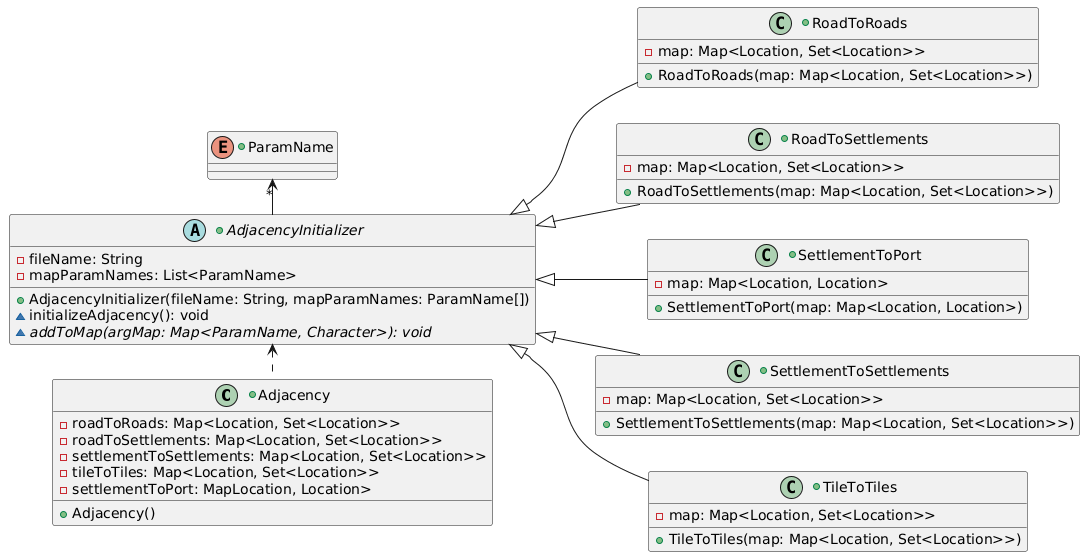
\includegraphics[width=\textwidth]{./duplicate_code.png}
Code for the \texttt{Adjacency} and \texttt{AdjacencyInitializer} classes and an example of one of the initializers:
\begin{lstlisting}[style=javacode,language=myJava]
public class Adjacency {
	private Map<Location, Set<Location>> roadToRoads;
	private Map<Location, Set<Location>> roadToSettlements;
	private Map<Location, Set<Location>> settlementToSettlements;
	private Map<Location, Set<Location>> tileToTiles;
	private Map<Location, Location> settlementToPort;
	
	public Adjacency() {
		roadToRoads = new HashMap<>();
		AdjacencyInitializer roadToRoadsInitializer = new RoadToRoads(roadToRoads);
		roadToRoadsInitializer.initializeAdjacency();
		
		settlementToSettlements = new HashMap<>();
		AdjacencyInitializer settlementToSettlementsInitializer = new
			SettlementToSettlements(settlementToSettlements);
		settlementToSettlementsInitializer.initializeAdjacency();

		roadToSettlements = new HashMap<>();
		AdjacencyInitializer roadToSettlementsInitializer = new 
			RoadToSettlements(roadToSettlements);
		roadToSettlementsInitializer.initializeAdjacency();

		tileToTiles = new HashMap<>();
		AdjacencyInitializer tileToTilesInitializer = new TileToTiles(tileToTiles);
		tileToTilesInitializer.initializeAdjacency();

		settlementToPort = new HashMap<>();
		AdjacencyInitializer settlementToPortInitializer = new 
			SettlementToPort(settlementToPort);
		settlementToPortInitializer.initializeAdjacency();

	public Set<Location> getRoadToRoads(Location roadLocation) {
		return this.roadToRoads.get(roadLocation);
	}

	public Set<Location> getRoadToSettlements(Location roadLocation) {
		return this.roadToSettlements.get(roadLocation);
	}

	public Set<Location> getSettlementToSettlements() {
		return this.settlementToSettlements.keySet();
	}

	public Set<Location> getSettlementToSettlements(Location settlementLocation) {
		return this.settlementToSettlements.get(settlementLocation);
	}

	public Set<Location> getTileToTiles(Location tileLocation) {
		return this.tileToTiles.get(tileLocation);
	}

	public Location getSettlementToPort(Location settlementLocation) {
		return this.settlementToPort.get(settlementLocation);
	}
}
\end{lstlisting}
\begin{lstlisting}[style=javacode,language=myJava]
public abstract class AdjacencyInitializer {
	private static final String ADJACENCY_RESOURCES_PATH = "src/main/resources/adjacency";

	private String fileName;
	private List<ParamName> mapParamNames;

	public AdjacencyInitializer(String fileName, ParamName[] mapParamNames) {
		this.fileName = fileName;
		this.mapParamNames = Arrays.asList(mapParamNames);
	}

	final void initializeAdjacency() {
		CatanFileReader fileReader = new CatanFileReader(
			new CatanScanner(ADJACENCY_RESOURCES_PATH, fileName));
		
		while (fileReader.hasNextLine()) {
			String line = fileReader.nextLine();
			List<Character> argList = Arrays.stream(line.split(","))
				.map(value -> value.charAt(0))
				.collect(Collectors.toList());
			Map<ParamName, Character> argMap = IntStream.range(0, mapParamNames.size())
				.boxed()
				.collect(Collectors.toMap(mapParamNames::get, argList::get));
			this.addToMap(argMap);
		}

		fileReader.close();
	}

	abstract void addToMap(Map<ParamName, Character> argMap);
}
\end{lstlisting}
\begin{lstlisting}[style=javacode,language=myJava]
public class SettlementToPort extends AdjacencyInitializer {
	static final ParamName paramNames[] =
		{ParamName.A, ParamName.B, ParamName.C, ParamName.P};

	private Map<Location, Location> map;

	@SuppressFBWarnings(
		value = "EI_EXPOSE_REP2",
		justification = "Need this to add to the map")
	public SettlementToPort(Map<Location, Location> map) {
		super("initializeSettlementToPort.txt", paramNames);
		this.map = map;
	}

	@Override
	void addToMap(Map<ParamName, Character> argMap) {
		Location settlement = new Location(argMap.get(ParamName.A), argMap.get(ParamName.B),
			argMap.get(ParamName.C));
		Location port = new Location(argMap.get(ParamName.P));

		map.put(settlement, port);
	}
}
\end{lstlisting}

\addcontentsline{toc}{section}{Large Method (Milestone 2)}
\section*{Large Method (Milestone 2)}
\subsection*{Description}
The \texttt{LocationChecker} class has many large methods with nested for loops and conditionals, making the methods less readable. The for loops and code inside the conditoinal blocks can be extracted into separate methods with names clearly indicating what they do. For example, with \texttt{getDefaultSettlementLocations}, we can extract a \texttt{findSettlementLocationsAdjacentToRoad} method and a \texttt{hasAdjacentSettlement} method. And in \texttt{getInitialRoadLocations}, we can replace conditionals hardcoded values with loops.
\subsection*{Before and After}
\subsubsection*{\texttt{getDefaultSettlementLocations}}
Before:
\begin{lstlisting}[style=javacode,language=myJava]
public Set<Location> getDefaultSettlementLocations(Color color) {
	Set<Location> settlementLocations = new HashSet<>();
	for (Location roadLocation : this.roads.get(color)) { // find all roads of color
		for (Location settlementLocation : this.adj.getRoadToSettlements(roadLocation)) {
				// adjacent settlements
			if (this.settlementPlacedAt(settlementLocation)) continue; // remove obstruction
			boolean closeSettlement = false;
			for (Location adjacentSettlement :
				this.adj.getSettlementToSettlements(settlementLocation)) {
				if (this.settlementPlacedAt(adjacentSettlement)) {
						// remove spots with adjacent settlements
					closeSettlement = true;
					break;
				}
			}
			if (!closeSettlement) {
				settlementLocations.add(settlementLocation);
			}
		}
	}
	return settlementLocations;
}
\end{lstlisting}
After:
\begin{lstlisting}[style=javacode,language=myJava]
public Set<Location> getDefaultSettlementLocations(Color color) {
	Set<Location> settlementLocations = new HashSet<>();
	for (Location roadLocation : this.roads.get(color)) {
		settlementLocations.addAll(this.findSettlementLocationsAdjacentToRoad(roadLocation));
	}
	return settlementLocations;
}

private Set<Location> findSettlementLocationsAdjacentToRoad(Location roadLocation) {
	Set<Location> settlementLocations = new HashSet<>();
	for (Location settlementLocation : this.adj.getRoadToSettlements(roadLocation)) {
		if (this.settlementPlacedAt(settlementLocation)) continue; // remove obstruction
		if (!this.hasAdjacentSettlement(settlementLocation)) {
			settlementLocations.add(settlementLocation);
		}
	}
	return settlementLocations;
}

private boolean hasAdjacentSettlement(Location location) {
	for (Location adjacentSettlement : this.adj.getSettlementToSettlements(location)) {
		if (this.settlementPlacedAt(adjacentSettlement)) {
			return true;
		}
	}
	return false;
}
\end{lstlisting}
\subsubsection*{\texttt{getInitialRoadLocations}}
Before:
\begin{lstlisting}[style=javacode,language=myJava]
public Set<Location> getInitialRoadLocations(Location settlement) {
	if (this.getRoads().size() >= 8) {}
		throw new IllegalStateException("cannot place more than 8 initial roads");
	}
	if (!this.getSettlements().contains(settlement)) {
		throw new IllegalStateException("cannot place road if settlement isn't placed");
	}
	char[] location = settlement.getArray();
	char a = location[0];
	char b = location[1];
	char c = location[2];
	Set<Location> roadLocations = new HashSet<>();
	if (!(isLowerCase(a) && isLowerCase(b))) { // coast settlements only have two roads
		roadLocations.add(new Location(a, b));
	}
	if (!(isLowerCase(b) && isLowerCase(c))) {
		roadLocations.add(new Location(b, c));
	}
	if (!(isLowerCase(a) && isLowerCase(c))) {
		roadLocations.add(new Location(a, c));
	}
	return roadLocations;
}
\end{lstlisting}
After:
\begin{lstlisting}[style=javacode,language=myJava]
public Set<Location> getInitialRoadLocations(Location settlement) {
	if (this.getRoads().size() >= 8) {
		throw new IllegalStateException("cannot place more than 8 initial roads");
	} else if (!this.getSettlements().contains(settlement)) {
		throw new IllegalStateException("cannot place road if settlement isn't placed");
	}

	char[] location = settlement.getArray();
	Set<Location> roadLocations = new HashSet<>();
	for (char a : location) {
		for (char b : location) {
			if (a != b && !(isLowerCase(a) && isLowerCase(b))) { // coast settlements only 
				have two roads
				roadLocations.add(new Location(a, b));
			}
		}
	}
	return roadLocations;
}
\end{lstlisting}
\subsubsection*{\texttt{isTileArrangementValid}}
Before:
\begin{lstlisting}[style=javacode,language=myJava]
public boolean isTileArrangementValid(Map<Location, Tile> tiles) {
	boolean isValid = true;
	for(Tile t : tiles.values()) {
		int number = t.getNumber();
		if(number == 6 || number == 8) {
			for(Location l : getAdjacentTiles(t.getLocation())) {
				int adjNumber = tiles.get(l).getNumber();
				if(adjNumber == 6 || adjNumber == 8) {
					isValid = false;
				}
			}
		}
	}
	return isValid;
}
\end{lstlisting}
After:
\begin{lstlisting}[style=javacode,language=myJava]
public boolean isTileArrangementValid(Map<Location, Tile> tiles) {
	boolean isValid = true; // flag to simplify mocking and improve test readability
	for(Tile t : tiles.values()) {
		int number = t.getNumber();
		if (number == 6 || number == 8) {
			if (this.hasAdjacent6Or8(tiles, t)) {
				isValid = false;
			}
		}
	}
	return isValid;
}
private boolean hasAdjacent6Or8(Map<Location, Tile> tiles, Tile t) {
	boolean hasAdjacent = false; // flag to simplify mocking and improve test readability
	for (Location l : getAdjacentTiles(t.getLocation())) {
		int adjNumber = tiles.get(l).getNumber();
		if (adjNumber == 6 || adjNumber == 8) {
			hasAdjacent = true;
		}
	}
	return hasAdjacent;
}
\end{lstlisting}
\subsubsection*{\texttt{getTilesAdjacentSettlement}}
Before:
\begin{lstlisting}[style=javacode,language=myJava]
public Set<Location> getTilesAdjacentToSettlement(Location settlementLocation) {
	char[] location = settlementLocation.getArray();
	char locA = location[0];
	char locB = location[1];
	char locC = location[2];
	Set<Location> tiles = new HashSet<>();
	if (!isLowerCase(locA)) {
		tiles.add(new Location(locA));
	}
	if (!isLowerCase(locB)) {
		tiles.add(new Location(locB));
	}
	if (!isLowerCase(locC)) {
		tiles.add(new Location(locC));
	}
	return tiles;
}
\end{lstlisting}
After:
\begin{lstlisting}[style=javacode,language=myJava]
public Set<Location> getTilesAdjacentToSettlement(Location settlementLocation) {
	Set<Location> tiles = new HashSet<>();
	for (char a : settlementLocation.getArray()) {
		if (!isLowerCase(a)) {
			tiles.add(new Location(a));
		}
	}
	return tiles;
}
\end{lstlisting}
\subsubsection*{\texttt{getLongestRoadForColor}}
Before:
\begin{lstlisting}[style=javacode,language=myJava]
public int getLongestRoadForColor(Color color) {
	Set<Integer> pathLengths = new HashSet<>();
	if(roads.get(color).isEmpty()) {
		return 0;
	}
	for(Location start : roads.get(color)) {
		for(Location road : adj.getRoadToRoads(start)) {
			if(this.roads.get(color).contains(road)) {
				boolean blocked = false;
				for(Location settlement : adj.getRoadToSettlements(road)) {
					if (settlementPlacedAt(settlement)
							&& !settlements.get(color).contains(settlement)
							&& adj.getRoadToSettlements(start).contains(settlement)) {
						blocked = true;
					}
				}
				if(!blocked) {
					Set<Location> seen = new HashSet<>();
					seen.add(start);
					pathLengths.add(longestRoadHelper(color, road, start, seen));
				}
			}
		}
	}
	if(pathLengths.isEmpty()) {
		return 1;
	}
	return 1 + Collections.max(pathLengths);
}

public int longestRoadHelper(Color color, Location road, Location previous,
		Set<Location> seen) {
	if(seen.contains(road)) {
		return 0;
	}
	Set<Integer> pathLengths = new HashSet<>();
	Set<Location> localSeen = new HashSet<>(seen);
	localSeen.add(road);
	for(Location adjacent : adj.getRoadToRoads(road)) {
		if(this.roads.get(color).contains(adjacent)
				&& !adj.getRoadToRoads(previous).contains(adjacent)){
			boolean blocked = false;
			for(Location settlement : adj.getRoadToSettlements(adjacent)) {
				if (settlementPlacedAt(settlement)
						&& !settlements.get(color).contains(settlement)
						&& adj.getRoadToSettlements(road).contains(settlement)) {
					blocked = true;
				}
			}
			if(!blocked) {
				pathLengths.add(longestRoadHelper(color, adjacent, road, localSeen));
			}
		}
	}
	return 1 + Collections.max(pathLengths);
}
\end{lstlisting}
After:
\begin{lstlisting}[style=javacode,language=myJava]
public int getLongestRoadForColor(Color color) {
	Set<Integer> pathLengths = new HashSet<>();
	if (roads.get(color).isEmpty()) {
		return 0;
	}

	for (Location start : roads.get(color)) {
		pathLengths.add(getLongestRoadFromStartLocation(color, start));
	}

	return 1 + getPathLengthsMax(pathLengths);
}

private int getLongestRoadFromStartLocation(Color color, Location start) {
	Set<Integer> pathLengths = new HashSet<>();
	for (Location road : adj.getRoadToRoads(start)) {
		if (roadWithSameColorIsAdjacent(color, road)) {
			if (!isBlocked(color, start, road)) {
				Set<Location> seen = new HashSet<>();
				seen.add(start);
				pathLengths.add(longestRoadHelper(color, road, start, seen));
			}
		}
	}
	return getPathLengthsMax(pathLengths);
}

public int longestRoadHelper(Color color, Location road, Location previous,
		Set<Location> seen) {
	if (seen.contains(road)) {
		return 0;
	}
	Set<Integer> pathLengths = new HashSet<>();
	Set<Location> localSeen = new HashSet<>(seen);
	localSeen.add(road);
	for (Location adjacent : adj.getRoadToRoads(road)) {
		if (roadWithSameColorIsAdjacent(color, adjacent)
				&& roadIsNotPreviousRoad(previous, adjacent)){
			if (!isBlocked(color, road, adjacent)) {
				pathLengths.add(longestRoadHelper(color, adjacent, road, localSeen));
			}
		}
	}
	return 1 + getPathLengthsMax(pathLengths);
}

private boolean roadIsNotPreviousRoad(Location previous, Location adjacent) {
	return !adj.getRoadToRoads(previous).contains(adjacent);
}

private boolean roadWithSameColorIsAdjacent(Color color, Location adjacent) {
	return this.roads.get(color).contains(adjacent);
}

private boolean isBlocked(Color color, Location previousLocation, Location road) {
	boolean blocked = false; // flag for testing because getRoadToSettlements returns a set
	for (Location settlement : adj.getRoadToSettlements(road)) {
		if (isBlockedBySettlement(color, previousLocation, settlement)) {
			blocked = true;
		}
	}
	return blocked;
}

private boolean isBlockedBySettlement(Color color, Location previousLocation,
		Location settlement) {
	return settlementPlacedAt(settlement) && !settlements.get(color).contains(settlement)
		&& adj.getRoadToSettlements(previousLocation).contains(settlement);
}
private int getPathLengthsMax(Set<Integer> pathLengths) {
	if (pathLengths.isEmpty()) {
		return 0;
	}
	return Collections.max(pathLengths);
}
\end{lstlisting}

\addcontentsline{toc}{section}{Temporary Field (Milestone 2)}
\section*{Temporary Field (Milestone 2)}
\subsection*{Description}
\texttt{Tile} has the temporary fields \texttt{number} and \texttt{typ}e since those fields are only used when \texttt{isDesert} is \texttt{false}, so when we want to find the \texttt{number} or \texttt{type} of a tile, we first need to check whether it is the desert.\\

\texttt{Port} has the temporary field \texttt{type}, which is only used when \texttt{generic} is \texttt{false}.\\

To fix both classes with temporary fields, we can add another \texttt{Type} called \texttt{NONE} and set \texttt{number} to \texttt{0}, which is an impossible value to roll. We can also add a constant for the resource types, which contains a subset of the types defined in \texttt{Type}.\\

Then, when we save the game state, we do not need to check if each tile or port to save is the desert or a generic port, and we can save the type.
\subsection*{Before}
\begin{lstlisting}[style=javacode,language=myJava]
public enum Type {
	WHEAT("wheat"),
	ORE("ore"),
	WOOL("wool"),
	BRICK("brick"),
	LUMBER("lumber");
	...
}
\end{lstlisting}
\begin{lstlisting}[style=javacode,language=myJava]
public class Tile {
	Location location;
	int number;
	Type type;
	
	boolean isDesert;

	public Tile(char location, int number, Type type) {
		assignLocation(location);
		setNumber(number);
		this.type = type;
		this.isDesert = false;
	}

	public Tile(char location) {
		assignLocation(location);
		this.number = 0;
		this.isDesert = true;
	}

	...

	public boolean getIsDesert() {
		return this.isDesert;
	}

	public boolean equals(Object other) {
		if (!(other instanceof Tile)) return false;
		if(this.isDesert || ((Tile)other).getIsDesert()) {
			return(this.location.equals(((Tile)other).getLocation())
				&& (this.number == ((Tile)other).getNumber()));
		}
		return(this.location.equals(((Tile)other).getLocation())
			&& (this.number == ((Tile)other).getNumber())
			&& (this.type.equals(((Tile)other).getType())));
	}

	...
}
\end{lstlisting}
\begin{lstlisting}[style=javacode,language=myJava]
public class Port {
	Location location; // default value
	boolean generic;
	Type type;

	public Port(Location location, Type type) {
		if(location.getArray()[0] < 'a') {
			throw new IllegalArgumentException("Invalid marker for location");
		}
		this.location = location;
		this.type = type;
		this.generic = false;
	}

	public Port(Location location) {
		if(location.getArray()[0] < 'a') {
			throw new IllegalArgumentException("Invalid marker for location");
		}
		this.location = location;
		this.type = null;
		this.generic = true;
	}

	public Port() {
		this(new Location('a'), Type.WHEAT);
	}

	...

	public void setGeneric() {
		generic = true;
	}

	public boolean isGeneric() {
		return generic;
	}

	...
}
\end{lstlisting}
\subsection*{After}
\begin{lstlisting}[style=javacode,language=myJava]
public enum Type {
	WHEAT("wheat"),
	ORE("ore"),
	WOOL("wool"),
	BRICK("brick"),
	LUMBER("lumber"),
	NONE("none");

	public static final Type[] RESOURCE_TYPES = new Type[]{WHEAT, ORE, WOOL, BRICK, LUMBER};
	...
}
\end{lstlisting}
\begin{lstlisting}[style=javacode,language=myJava]
public class Tile {
	Location location;
	int number;
	Type type;

	public Tile(char location, int number, Type type) {
		assignLocation(location);
		setNumber(number);
		this.type = type;
	}

	public Tile(char location) {
		assignLocation(location);
		this.number = 0; // impossible to roll 0
		this.type = Type.NONE;
	}

	...

	public boolean getIsDesert() {
		return this.type == Type.NONE;
	}

	public boolean equals(Object other) {
		if (!(other instanceof Tile)) return false;
		if(this.type == Type.NONE || ((Tile)other).getIsDesert()) {
			return(this.location.equals(((Tile)other).getLocation())
				&& (this.number == ((Tile)other).getNumber()));
		}
		return(this.location.equals(((Tile)other).getLocation())
			&& (this.number == ((Tile)other).getNumber())
			&& (this.type.equals(((Tile)other).getType())));
	}

	...
}
\end{lstlisting}
\begin{lstlisting}[style=javacode,language=myJava]
public class Port {
	Location location; // default value
	Type type;
	
	public Port(Location location, Type type) {
		if(location.getArray()[0] < 'a') {
			throw new IllegalArgumentException("Invalid marker for location");
		}
		this.location = location;
		this.type = type;
	}

	public Port(Location location) {
		this(location, Type.NONE);
	}

	...

	public void setGeneric() {
		this.type = Type.NONE;
	}

	public boolean isGeneric() {
		return type == Type.NONE;
	}

	...
}
\end{lstlisting}

\addcontentsline{toc}{section}{Speculative Generality (Milestone 3)}
\section*{Speculative Generality (Milestone 3)}
\subsection*{Description}
The datasource layer has a \texttt{Loader} Interface, so that other types of loaders, besides file loaders could be used. We only use one type of loader, so we do not need the \texttt{Loader} interface. Also, the methods in the \texttt{Loader} interface seemed specific to loading from a file or would require other loaders to give information to the game in a way similar to reading from a file.
\subsection*{Before}
\texttt{Loader}:
\begin{lstlisting}[style=javacode,language=myJava]
boolean hasNextLine();
String nextLine();
void close();
\end{lstlisting}
\texttt{CatanLoader}:
\begin{lstlisting}[style=javacode,language=myJava]
private CatanScanner scanner;

public CatanLoader(CatanScanner scanner) {
	this.scanner = scanner;
}

public boolean hasNextLine() {
	return scanner.hasNextLine();
}

public String nextLine() {
	if (!hasNextLine()) throw new NoSuchElementException("No line found");
	return scanner.nextLine();
}

public void close() {
	scanner.close();
}
\end{lstlisting}
\texttt{FileLoaderImporter}:
\begin{lstlisting}[style=javacode,language=myJava]
private FileLoader loader;

public FileLoaderImporter(File file) {
	loader = new FileLoader(file);
}
\end{lstlisting}
\subsection*{After}
\texttt{FileLoader}(renamed from \texttt{CatanLoader}):
\begin{lstlisting}[style=javacode,language=myJava]
private CatanScanner scanner;

public FileLoader(CatanScanner scanner) {
	this.scanner = scanner;
}

public boolean hasNextLine() {
	return scanner.hasNextLine();
}

public String nextLine() {
	if (!hasNextLine()) throw new NoSuchElementException("No line found");
	return scanner.nextLine();
}

public void close() {
	scanner.close();
}
\end{lstlisting}
\texttt{FileLoaderImporter}:
\begin{lstlisting}[style=javacode,language=myJava]
private FileLoader loader;

public FileLoaderImporter(File file) {
	loader = new FileLoader(CatanScanner.createCatanScanner(file));
}

public void importGame() {
	while (loader.hasNextLine()) {
		System.out.println(loader.nextLine());
	}
}
\end{lstlisting}
\end{document}
